\section{Contexto e motivação}
Nesta secção deve explicar de forma clara a relevância do trabalho proposto. Para tal deve enquadrá-lo, apresentando as razões pelas quais a realização deste trabalho é importante.

\section{Objetivos}
Nesta secção deve apresentar de forma clara os objetivos de trabalho.

\section{Contribuições}
Nesta secção deve apresentar as contribuições do trabalho, dando especial relevo às que são novidade. Note que a inovação não é obrigatória em trabalhos de mestrado. Portanto nesta secção deve descrever sucintamente todo o trabalho realizado.

\section{Organização da dissertação (opcional)}
Nesta secção deve descrever sucintamente como a dissertação está organizada.

\section{Como utilizar este template}
Esta secção serve para dar algumas instruções sobre a edição de textos em latex e utilização deste template.

\subsection{Software necessário}
Para editar textos em latex no windows necessita de instalar o seguinte software:
\begin{itemize}
  \item Miktex 2.9 - fazer download em https://miktex.org/download e seguir instruções de instalação;
  \item Instalar os seguintes pacotes do Miktex: acronym, emptypage, epigraph, tocbibind, titlesec, ifoddpage, algcompatible, algpseudocode; Estes pacotes serão fornecidos no e-learning;
  \item Winedt 10 - fazer download em http://www.winedt.com/download.html e seguir instruções de instalação.
\end{itemize}

Em alternativa ao winedt poderá utilizar o kile para linux.


\subsubsection{Como instalar os pacotes do Miktex}
Para instalar os pacotes disponíveis na página do e-learning deve seguir os seguintes passos:
\begin{enumerate}
  \item Copiar as diretorias descompactadas para C:$\setminus$ Program Files (x86)$\setminus$ MiKTeX 2.9$\setminus$ tex$\setminus$ latex;
  \item No windows fazer start-> MiKTeX 2.9 -> MiKTeX Settings (admin) -> Clicar em Refresh FNDB no separador General.
\end{enumerate}

\subsection{Como utilizar o template Tese-IPT}
O template Tese-IPT está de acordo com as regras estabelecidas para a realização de dissertações de mestrado. A capa é feita à parte e inserida como pdf (ver código ficheiro main).

O template Tese-IPT é constituído pelos seguintes ficheiros:
\begin{itemize}
  \item main.tex - ficheiro tex principal;
  \item xxxx.tex - ficheiros tex de cada capítulo;
  \item ficheiros com as imagens inseridas na dissertação que se encontram na diretoria images;
  \item references.bib - ficheiro com as referências bibliográficas.
\end{itemize}
Para criar o documento deve abrir o ficheiro main.tex com o winedt e depois clicar no ícone PDFLaTeX. Para ver o ficheiro PDF deve clicar no ícone PDF Preview.

Para inserir novos capítulos deve criar um novo ficheiro .tex e guardá-lo na mesma diretoria do main. Depois basta inseri-lo utilizando a mesma forma utilizada para inserir os capítulos, Introdução, Estado da Arte e Conclusão já inseridos no ficheiro main.tex.

\subsection{Exemplos de como fazer figuras}
Para incluir uma figura no texto deve utilizar o objecto figure (Insert->Object->Figure).
\begin{figure}[ht]
  \centering
  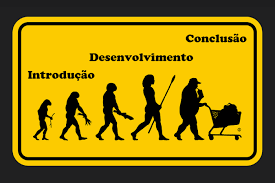
\includegraphics[width=0.5\textwidth]{images/figura1.png}
  \caption{Figura cuja largura é metade da largura do texto. Também pode utilizar o comando scale}\label{fig1}
\end{figure}
Para referir a figura anterior deve-se usar o label da figura e o comando ref (Fig. \ref{fig1}). Pode-se usar os comandos h (here), ht (heretop), t(top) ,b(bottom) para colocar as figuras no cimo da página, no fundo da página ou naquele preciso local. O comando caption serve para colocar a legenda da figura. Note-se que o índice de figuras é atualizada automaticamente.

Para colocar figuras ao lado umas das outras pode usar o ambiente minipage (disponível no pacote subcaption). a Fig. \ref{fig2} é resultado da aplivação do ambiente minipage.

\begin{figure}[htbp]
\centering
\begin{minipage}{0.35\textwidth}
  \centering
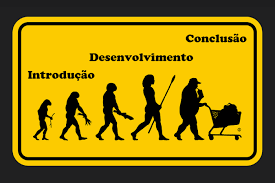
\includegraphics[width=0.35\textwidth]{images/figura1.png}
\subcaption[first caption.]{Primeira figura...}\label{fig2a}
\end{minipage}%
\begin{minipage}{0.35\textwidth}
  \centering
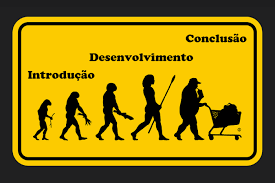
\includegraphics[width=0.35\textwidth]{images/figura1.png}
\subcaption[second caption.]{Segunda figura...}\label{fig2b}
\end{minipage}%
\begin{minipage}{0.35\textwidth}
  \centering
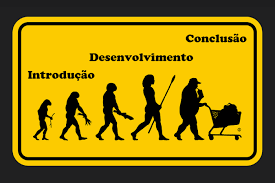
\includegraphics[width=0.35\textwidth]{images/figura1.png}
\subcaption[third caption.]{Terceira figura...}\label{fig2c}
\end{minipage}

\caption{Legenda geral da figura} \label{fig2}
\end{figure}

\subsubsection{Exemplos de Tabelas}

Para fazer tabelas deve inserir um objeto Table e dentro desse objeto deve incluir um objeto tabular. A tabela \ref{tab1} mostra um primeiro exemplo de como uma tabela simples.

\begin{table}[h]
  \centering
    \begin{tabular}{|l|c|c|c|c|c|}\hline
    % after \\: \hline or \cline{col1-col2} \cline{col3-col4} ...
    a & b & c & d & e & f \\\hline 
    1 & 5 & 9 & 4 & 8 & 3 \\\hline 
    2 & 6 & 1 & 5 & 9 & 4 \\\hline 
    3 & 7 & 2 & 6 & 1 & 5 \\\hline 
    4 & 8 & 3 & 7 & 2 & 6 \\\hline
    \end{tabular}
    \caption{Tabela realizada com array}\label{tab1}
\end{table}

A tabela \ref{tab2} mostra um segundo exemplo de como fazer tabelas.

\begin{table}[h]
  \centering
    \begin{tabular}{cccccc}\hline
    % after \\: \hline or \cline{col1-col2} \cline{col3-col4} ...
    a & b & c & d & e & f \\\hline\hline
    1 & 5 & 9 & 4 & 8 & 3 \\\hline
    2 & 6 & 1 & 5 & 9 & 4 \\\hline
    3 & 7 & 2 & 6 & 1 & 5 \\\hline
    4 & 8 & 3 & 7 & 2 & 6 \\\hline
    \end{tabular}
    \caption{Outra tabela ....}\label{tab2}
\end{table}

A tabela \ref{tab3} mostra um terceiro exemplo de como fazer tabelas.

\begin{table}[!htpb]
\centering

% definir o tamanho da fonte para small
% outros possíveis tamanhos: footnotesize, scriptsize
\begin{small}
% redefinindo o espaçamento das colunas
\setlength{\tabcolsep}{3pt}
% \cline é semelhante ao \hline, porém é possível indicar as colunas que terão essa a linha horizontal
% \multicolumn{10}{c|}{Meses} indica que dez colunas serão mescladas e a palavra Meses estará centralizada dentro delas.
\begin{tabular}{|c|c|c|c|c|c|c|c|c|c|c|c|c|c|c|c|c|c|c|c|c|c|c|c|c|}\hline
 & \multicolumn{24}{c|}{Meses}\\ \cline{2-25}
\raisebox{1.5ex}{Etapa} & 01 & 02 & 03 & 04 & 05 & 06 & 07 & 08 & 09 & 10 & 11 & 12 & 13 & 14 & 15 & 16 & 17 & 18 & 19 & 20 & 21 & 22 & 23 & 24 \\ \hline
1 & X & X & X & X & X & X & X & X & X & X & X & X & & & & & & & & & & & & \\ \hline
2 & & X & X & X & X & X & X & X & X & X & X & X & & & & & & & & & & & & \\ \hline
3 & & X & X & X & X & X & X & X & X & X & X & X & X & X & X & X & X & X & X & X & & & & \\ \hline
4 & & X & X & X & X & X & X & X & X & X & X & X & X & X & X & X & X & X & X & X & & & & \\ \hline
5 & & X & X & X & X & X & X & X & X & X & X & X & X & X & X & X & & & & & & & & \\ \hline
6 & & X & X & X & X & X & X & X & X & X & X & X & X & X & X & X & X & X & X & X & X & & & \\ \hline
7 & & & & X & X & X & X & X & X & X & X & X & X & X & X & X & X & X & X & X & X & X & & \\ \hline
8 & & & & & & X & X & X & X & X & X & X & X & X & X & X & X & X & X & X & X & X & X & X \\ \hline
\end{tabular}
\end{small}
\caption{Cronograma das atividades previstas}
\label{tab3}
\end{table} 

\cleardoublepage 

\subsubsection{Equações}

De seguida apresentam-se exemplos de como fazer e referenciar equações em latex. Em (\ref{eq1}) pode ver o exemplo de uma equação simples.
\begin{equation}\label{eq1}
  x=\frac{1+y}{1+2z^2}
\end{equation}
Em (\ref{eq2}) te o exemplo de uma equação mais complexa com fracções.
\begin{equation}\label{eq2}
 \frac{1}{\displaystyle 1+
   \frac{1}{\displaystyle 2+
   \frac{1}{\displaystyle 3+x}}} +
 \frac{1}{1+\frac{1}{2+\frac{1}{3+x}}}
\end{equation}
A equação (\ref{eq3}) mostra como pode escrever e incluir espaços dentro do ambiente equation.
\begin{equation}\label{eq3}
  x_1 = a+b ~~\mbox{and}~~ x_2=a-b
\end{equation}
O último exemplo em (\ref{eq4}) mostra como pode colocar equações em várias linhas.
\begin{eqnarray}\label{eq4}
 y &=& x^4 + 4      \nonumber \\
   &=& (x^2+2)^2 -4x^2 \nonumber \\
   &\le&(x^2+2)^2
\end{eqnarray}
Note que pode simplesmente fazer uma equação entre dois cifrões não sendo para tal necessário utilizar os ambientes exemplificados anteriormente. Por exemplo, a equação feral da dinâmica diz-nos que $F=m\times a$, onde $F$ representa a Força, $m$ a massa e $a$ a aceleração.

Em \cite{CEU2017} pode ver mais exemplos de equações editadas em latex. 

\subsubsection{Referências}
Para as referências este template utiliza o ficheiro reference.bib. Para adicionar referências deve seguir os seguintes passos:
\begin{itemize}
  \item Inserir a referência no ficheiro reference utilizando um dos BiBTeX items à escolha;
  \item No texto incluir a referência utilizando o comando $\setminus$cite.
  \item No ficheiro principal correr o comando pdflatex;
  \item No ficheiro principal correr o comando bibtex.
\end{itemize}
Em \cite{Oliveira11wirelesssensor} pode ver um exemplo de citação de um artigo de revista, em \cite{Lopes2011} pode ver um exemplo de citação de um artigo de conferência e em \cite{Ferreira2015} pode ver a referência de uma tese. 

